\section{Exact transfer through survivor corridors}
\label{sec:survivor-corridors}

The principal new reduction in this article evaluates only those algebraic
paths that can connect surviving generators.  It can evaluate a connected
part of the transfer from either its sources or its targets, and chooses the
direction from a precise count of possible coefficient propagations.  The
result is the full minimal differential, including its nonzero radical
entries.  No homology rank is inferred merely from the number of survivors.

The distinction from the preceding work is essential.  The scalar-residue
profile, the recovered quantum grading, and homological perturbation transfer
are earlier results of this project.  A preceding local prototype already
implemented a complete forward quantum sweep and checked its contraction
identities.  We preserve that prototype as a frozen reference and retain its
scalar basis convention.  The new results are the corridor restriction, its
typed support refinement, componentwise choice of transfer direction, and
families exhibiting unbounded improvements in the corresponding transfer
operation counts.  Neither homological perturbation nor dynamic programming
on a directed acyclic graph is claimed as a new general technique.

\subsection{Homogeneous maps and the scalar contraction}

Fix a frontier with $2k$ endpoints.  Write $a,b$ for matching objects and
$c(a,b)$ for the number of circles in their overlay.  In the coefficient model
of the scanner, a basis of $\operatorname{Hom}(a,b)$ consists of the squarefree
dot monomials on these circles.  A monomial containing $r$ dots has intrinsic
weight
\begin{equation}\label{eq:corridor-intrinsic-weight}
  \omega=k-c(a,b)+2r,\qquad 0\le r\le c(a,b).
\end{equation}
Its possible weights therefore form the finite set
\begin{equation}\label{eq:corridor-weight-set}
  \mathcal W(a,b)=
  \{k-c(a,b),k-c(a,b)+2,\ldots,k+c(a,b)\}.
\end{equation}
In particular, every weight is nonnegative.  Since $c(a,b)=k$ holds precisely
when $a=b$, weight zero consists only of scalar identities between copies of
the same matching.

An object in the chain complex has a homological degree $h$ and a quantum
shift $q$.  The grading convention is that a differential entry from
$(a,h,q)$ to $(b,h+1,q')$ has intrinsic weight $q'-q$.  The shifts in the
ordinary scanner, although previously erased from its stored state, are
recovered by the recurrence
\begin{equation}\label{eq:corridor-q-recurrence}
 q_{\mathrm{child}}=q_{\mathrm{parent}}+\epsilon+\ell-2|L|.
\end{equation}
Here $\epsilon\in\{0,1\}$ is the smoothing, $\ell$ is the number of circles
created by that smoothing, and $L$ is the subset selected by the delooping
label.  Preservation of this grading by gluing, delooping, and cancellation
is supplied by the preceding recovered-grading analysis.  The new scanner
subclass stores these shifts explicitly.

Let $d_0$ retain only the scalar identity entries of $d$, and put
$\delta=d-d_0$.  Projection to weight zero is multiplicative, so $d_0^2=0$.
Moreover,
\begin{equation}\label{eq:corridor-positive-delta}
 \delta_{ba}\ne0\quad\Longrightarrow\quad q_b>q_a.
\end{equation}
A unit in a homogeneous differential is exactly $1$: a dotted term has
positive weight and cannot occur in the same homogeneous coefficient as its
scalar term.  Thus nonhomogeneous synthetic inputs with coefficients such as
$1+x$ are outside the assumptions of this reducer.

For each matching and quantum shift separately, choose a binary decomposition
\begin{equation}\label{eq:corridor-bhl}
 C^h=B^h\oplus H^h\oplus L^h,
 \qquad B^h=\operatorname{im}d_0^{h-1},\qquad
 \ker d_0^h=B^h\oplus H^h.
\end{equation}
Choose the basis of $B^{h+1}$ to be the images under $d_0$ of the basis of
$L^h$.  Then $d_0:L^h\to B^{h+1}$ is represented by an identity matrix.
Let $i$ include $H$, let $p$ project onto $H$, and let $h$ send the chosen
boundary basis to its chosen lifts in $L$, vanishing on $H$ and $L$.

\begin{lemma}[Typed binary contraction]\label{lem:corridor-binary}
The maps $i,p,h$ preserve matching type and quantum shift.  They satisfy
\begin{align}
 pi&=1,&d_0h+hd_0&=1+ip,\label{eq:corridor-scalar-main}\\
 h^2&=0,&hi&=0,&ph&=0,&d_0i&=0,&pd_0&=0.
 \label{eq:corridor-scalar-side}
\end{align}
They can be computed by binary linear algebra, without any cobordism
composition.
\end{lemma}

\begin{proof}
All complements and bases are chosen within a fixed matching and quantum
shift.  Every nonzero matrix coefficient of $i,p,h$ is therefore an identity
of that matching.  On $H$, the map $ip$ is the identity and both $d_0h$ and
$hd_0$ vanish.  On $B$, the composite $d_0h$ is the identity and $hd_0$ vanishes.
On $L$, the composite $hd_0$ is the identity and $d_0h$ vanishes.  These three
calculations give~\eqref{eq:corridor-scalar-main} in characteristic two.
The image of $h$ lies in $L$, where $h$ and $p$ vanish; $h$ also vanishes on
$H$.  This proves the first three side conditions.  The last two follow
because $i$ lands in cycles and $p$ kills boundaries.  Images, kernels,
complements, and the inverse of the resulting basis matrix are all computed
over $\mathbb F_2$.
\end{proof}

The dimensions of $H$ are the graded scalar-residue survivor profile.  If
$m_{a,h,q}$ is the original multiplicity and $r_{a,h,q}$ is the rank of the
corresponding scalar differential, then
\begin{equation}\label{eq:corridor-profile}
 \mu_{a,h,q}=m_{a,h,q}-r_{a,h,q}-r_{a,h-1,q}.
\end{equation}
These multiplicities do not depend on the chosen binary basis.  The support
of $i,p,h$, and hence the size of the transfer graph below, generally does.

\subsection{Why quantum transfer needs no radical-depth guess}

Because $h$ preserves quantum shift and $\delta$ strictly raises it,
$h\delta$ is nilpotent on a finite complex.  If its occupied shifts lie
between $q_{\min}$ and $q_{\max}$, the coarse bound
$(h\delta)^{q_{\max}-q_{\min}+1}=0$ suffices.  The empty complex is handled
separately and has zero transfer.  Consequently all inverses in the following
formulas are finite geometric sums:
\begin{align}
 I'&=(1+h\delta)^{-1}i,&
 D&=p\delta(1+h\delta)^{-1}i,\label{eq:corridor-transfer}\\
 P'&=p(1+\delta h)^{-1},&
 H'&=h(1+\delta h)^{-1}.
 \label{eq:corridor-transfer-maps}
\end{align}
These are the finite specialization of the homological perturbation formulas \cite{Crainic2004}.
They give a special contraction from $(C,d)$ to $(H,D)$:
\begin{align}
 dI'&=I'D,&P'd&=DP',&P'I'&=1,\label{eq:corridor-cert-chain}\\
 dH'+H'd&=1+I'P',&H'^2&=0,&H'I'&=0,&P'H'&=0,&D^2&=0.
 \label{eq:corridor-cert-homotopy}
\end{align}
The inherited reference computes all four maps when requested and checks
these eight identities in the actual coefficient algebra.  The new reduction
computes only $D$ during ordinary execution; its tests compare $D$ entry by
entry with that fully certified reference in the same scalar basis.

The quantum proof is useful for the scope of the implementation.  It does
not use an assumed common cyclic order on a catalogue of abstract matching
objects or an assumed sharp radical exponent for that catalogue.  The maps
being composed are entries of the valid input complex and scalar identities
between copies of the same matching.  Every transfer path composes them in
their given order.  Thus the argument requires the same legitimate typed
cobordism compositions as ordinary Gaussian cancellation.  It does not
license geometrically impossible tables or independently verify the entire
underlying cobordism implementation.

There is also a direct block-matrix interpretation.  In the basis of
\eqref{eq:corridor-bhl}, the paired $L$-to-$B$ block of the differential is
$1+A$, where $A$ strictly raises quantum shift.  With $U$ the $H$-to-$B$
block, $V$ the $L$-to-$H$ block, and $W$ the direct $H$-to-$H$ block, the
surviving Schur complement is
\begin{equation}\label{eq:corridor-schur}
 D=W+V(1+A)^{-1}U.
\end{equation}
This is ordinary cancellation expressed as a finite triangular solve.  Its
entries have positive weight, so no scalar unit remains.  In particular, its
objects are exactly the survivors~\eqref{eq:corridor-profile}; retaining
those objects while discarding $D$ would in general be incorrect.

\subsection{A graph whose path sum is the minimal differential}

Fix a homological degree $h$.  The transfer of $D^h:H^h\to H^{h+1}$ uses
only the following graph.  For each original degree-$h$ object $a$, introduce
a vertex $z_a$.  For each original degree-$(h+1)$ object $b$, introduce a
vertex $w_b$.  There is an input port $s$ for each chosen survivor in $H^h$
and an output port $t$ for each chosen survivor in $H^{h+1}$.  The four kinds
of edges, excluding zero coefficients, are
\begin{equation}\label{eq:corridor-edges}
\begin{array}{ccl}
 s\longrightarrow z_a&\text{if }i_{as}=1,&\text{scalar identity},\\
 z_a\longrightarrow w_b&\text{if }\delta_{ba}\ne0,&\text{coefficient }\delta_{ba},\\
 w_b\longrightarrow z_a&\text{if }h_{ab}=1,&\text{scalar identity},\\
 w_b\longrightarrow t&\text{if }p_{tb}=1,&\text{scalar identity}.
\end{array}
\end{equation}
The letters $z,w$ distinguish intermediate positions in a matrix product;
they are not new chain objects.  Every path carries the ordered composite of
its edge coefficients.  Scalar identities have matching types compatible
with their incident vertices.

\begin{lemma}[Quantum acyclicity]\label{lem:corridor-acyclic}
The graph~\eqref{eq:corridor-edges} is directed and acyclic.  Its internal
vertices can be topologically ordered by quantum shift, placing $w$ before
$z$ at equal shift.
\end{lemma}
\begin{proof}
A radical edge $z_a\to w_b$ strictly raises $q$ by
\eqref{eq:corridor-positive-delta}.  A homotopy edge $w_b\to z_a$ preserves
$q$ and increases the indicated phase.  Input edges enter $z$ and output
edges leave $w$, so the terminal ports can be inserted in a compatible order.
For example, at equal shift the order $w,s,z,t$ works.  Every edge then goes
strictly forward in the lexicographic order on shift and phase.
\end{proof}

\begin{theorem}[Exact transfer path sum]\label{thm:corridor-pathsum}
For input $s$ and output $t$, the entry $D^h_{ts}$ is the sum over
$\mathbb F_2$ of the ordered cobordism products along all directed paths
from $s$ to $t$ in~\eqref{eq:corridor-edges}.
\end{theorem}
\begin{proof}
Expand the finite inverse in~\eqref{eq:corridor-transfer}:
\[
 D=\sum_{r\ge0}p\delta(h\delta)^ri.
\]
The summand with index $r$ is a matrix product.  Expanding its entries sums
over an inclusion edge, $r+1$ radical edges, $r$ homotopy edges, and a
projection edge, with their intermediate indices matched in order.  These
are precisely the graph paths with $r$ homotopy edges.  Conversely every
input-output path has this alternating form.  Acyclicity makes the total
number of paths finite, and each occurs once in the expansion.  Thus the
two sums have exactly the same terms, with the same multiplication order.
\end{proof}

The theorem concerns a path \emph{sum}.  It does not assert that the product
of every graph path is nonzero, or that different paths make distinct
contributions.  Two dots can annihilate a product, surface relations can
annihilate it, and equal contributions can cancel modulo two.  The graph
is a safe structural description of possible work, not a numerical rank
computation.

\subsection{Removing every branch irrelevant to survivors}

For a graph vertex $v$, let $L(v)$ be the set of input ports from which $v$
is reachable, and let $R(v)$ be the set of output ports reachable from $v$.
These sets are computed by ordinary unions of packed Boolean labels in
forward and reverse topological order.  They are not computed by XOR.

\begin{definition}[Survivor corridor]\label{def:corridor}
The survivor corridor is the subgraph consisting of the vertices and edges
lying on at least one input-output path.  Equivalently, retain vertices with
$L(v)\ne\varnothing$ and $R(v)\ne\varnothing$, and retain the edges between
them.
\end{definition}

The equivalence for edges follows directly: if an edge joins a vertex
reachable from an input to a vertex that can reach an output, concatenating
those paths with the edge gives an input-output path.

\begin{theorem}[Exact corridor restriction]\label{thm:corridor-pruning}
Replacing the complete transfer graph by its survivor corridor leaves every
entry of $D^h$ unchanged.  If its corridor is empty, then $D^h=0$.
\end{theorem}
\begin{proof}
Every path contributing to the sum of Theorem~\ref{thm:corridor-pathsum}
lies entirely in the corridor by its definition.  Conversely a path in the
retained graph is still a path in the original graph.  The two finite path
sums are therefore identical term by term.  An empty corridor has no terms.
\end{proof}

This zero certificate uses more information than the survivor profile.  For
example, a survivor can map into a scalar-contractible branch from which no
output survivor is reachable.  The survivor degrees and matching types may
permit a radical output map, but that branch makes no contribution to it.
Theorem~\ref{thm:corridor-pruning} removes it before evaluating its products.

The weakly connected components of the corridor, \emph{including its terminal
ports}, give independent blocks of $D^h$.  Indeed, every directed path lies
in one weak component, and no terminal belongs to two such components.
Sources or targets that belong to no corridor contribute zero columns or
rows.  The statement is degreewise: to decompose the complete reduced chain
complex into direct summands, the nonzero differential blocks in all adjacent
degrees must be taken into account.

\subsection{Typed support gives an additional exact restriction}

The grading supplies an inexpensive obstruction to a path product even when
the underlying graph path exists.  A prefix from survivor $s$ to vertex $v$
is homogeneous of weight $q_v-q_s$.  Its source and target matchings are
$m_s,m_v$, respectively.  Formula~\eqref{eq:corridor-weight-set} therefore
imposes a range and parity condition on that prefix.

\begin{proposition}[Typed prefix and suffix pruning]
\label{prop:corridor-typed}
A prefix from $s$ to $v$ evaluates to zero if
$q_v-q_s\notin\mathcal W(m_s,m_v)$.  A suffix from $v$ to $t$ evaluates to
zero if $q_t-q_v\notin\mathcal W(m_v,m_t)$.  Removing a path with either
property preserves the transfer exactly.  In particular, no nonzero prefix
or suffix has quantum weight greater than $2k$.
\end{proposition}
\begin{proof}
The edge coefficients are homogeneous and their intrinsic weights add under
valid composition.  Along a prefix the intermediate shifts telescope, leaving
$q_v-q_s$.  But the homogeneous part of the stated Hom space is zero outside
\eqref{eq:corridor-weight-set}.  The suffix calculation is the same.  A full
path with a zero prefix or suffix has zero product by associativity, so its
removal cannot alter the sum.  Finally $k+c(a,b)\le2k$.
\end{proof}

One implementation can test this condition immediately before attempting a
coefficient composition.  A stronger preprocessing option propagates input
labels while deleting labels forbidden by the Hom weight at each vertex,
and propagates output labels dually.  This remains a Boolean overestimate:
it does not attempt to decide cancellation among different allowed paths.
The production measurements reported here use structural corridor pruning;
the typed refinement is a proved extension and is not silently included in
their measured operation reductions.

The same support observation strengthens the older zero-differential profile
certificate.  Between survivors $(a,h,q)$ and $(b,h+1,q')$, a nonzero minimal
map is possible only when
\begin{equation}\label{eq:corridor-survivor-admissibility}
 \Delta=q'-q>0,\qquad
 k-c(a,b)\le\Delta\le k+c(a,b),\qquad
 \Delta\equiv k-c(a,b)\pmod 2.
\end{equation}
If no pair of adjacent-degree survivors satisfies these conditions, the
entire minimal differential is zero.  This is a sufficient certificate,
not a necessary condition: the actual maps can vanish for additional
algebraic reasons.  It is implemented as a separate reference strategy so
that its benefit can be measured independently of complete transfer.

\subsection{Forward and reverse evaluation}

For a fixed input survivor, forward evaluation accumulates its prefix
coefficients in topological order.  At a radical edge $u\to v$ carrying $f$,
it composes $f$ after the current prefix at $u$ and adds the result at $v$.
Scalar edges copy and add.  The coefficients arriving at output ports form
one column of $D^h$.

For a fixed output survivor, reverse evaluation starts with its projection
incidence and accumulates suffix coefficients in reverse topological order.
At a radical edge $u\to v$, it composes the current suffix at $v$ after $f$
and adds the result at $u$.  The multiplication order is important: this is
not an assumption that arbitrary cobordism coefficients commute.  The
coefficients arriving at inputs form one row of $D^h$.

\begin{theorem}[Bidirectional corridor transfer]
\label{thm:corridor-bidirectional}
Forward and reverse evaluation compute exactly the same minimal
differential.  Either orientation may be chosen separately for each weak
component of the survivor corridor.
\end{theorem}
\begin{proof}
Both evaluations compute the finite path sum of
Theorem~\ref{thm:corridor-pathsum}.  Forward evaluation groups its terms by
their initial portions, while reverse evaluation groups them by their final
portions.  Associativity identifies each complete ordered product, and
bilinearity permits the indicated grouping of sums.  A directed path cannot
cross between distinct weak components, so the choices for separate blocks
do not interact.
\end{proof}

\subsection{What the direction choice provably minimizes}

For one weak component $G_j$ of the corridor, define
\begin{equation}\label{eq:corridor-unit-bounds}
 F_j=\sum_{e:u\to v\in G_j}|L(u)|,
 \qquad
 B_j=\sum_{e:u\to v\in G_j}|R(v)|.
\end{equation}
Input and output incidence edges are included in these sums.  In the forward
algorithm, an edge can be processed for input $s$ only if $s\in L(u)$;
in the reverse algorithm, it can be processed for output $t$ only if
$t\in R(v)$.  Algebraic zero tests and cancellations can reduce the actual
numbers of processed edges.

\begin{theorem}[Certified propagation bound]\label{thm:corridor-work}
Choose forward evaluation when $F_j\le B_j$ and reverse evaluation otherwise.
Then the number of coefficient-edge propagations is at most
\begin{equation}\label{eq:corridor-total-propagations}
  \sum_j\min(F_j,B_j).
\end{equation}
If $a_j,b_j$ are the numbers of input and output ports and $E_j$ is the
number of edges in $G_j$, a coarser bound is
\begin{equation}\label{eq:corridor-coarse-propagations}
 \sum_j\min(a_j,b_j)E_j.
\end{equation}
\end{theorem}
\begin{proof}
For a fixed input, nonzero accumulated data at $u$ implies the existence of
at least one graph path from that input to $u$.  Thus it causes at most one
propagation of $e$ for a label in $L(u)$, and no others.  Summing over inputs
and edges proves the forward bound.  The reverse bound is identical with
suffixes.  The implemented choice gives their minimum for every component.
Finally $|L(u)|\le a_j$ and $|R(v)|\le b_j$, which gives
\eqref{eq:corridor-coarse-propagations}.
\end{proof}

This is an exact structural upper bound for a specified count, not a wall
clock oracle.  A radical edge may require a cobordism product; a scalar edge
requires only a coefficient copy or XOR.  The implementation also bypasses
composition by a correctly typed identity and reuses coefficient caches.
Consequently different propagations need not have equal observed costs.

To express a bit bound, let $\beta(k)=O(2^k)$ bound a coefficient copy/XOR
and let $\kappa(k)$ bound a full coefficient composition at this frontier.
The available dense kernel supplies a conservative
$\kappa(k)=\operatorname{poly}(k)2^k$ bound, with the usual additional cost
for normalized labels.  Multiplying~\eqref{eq:corridor-total-propagations}
by $\max(\beta(k),\kappa(k))$ bounds the coefficient work of the implemented
unit-weight choice.

A possible refinement assigns an edge cost $c_e$, for example
$\kappa(k)$ on radical edges and $\beta(k)$ on scalar edges, and chooses
between
\[
 F_j^{(c)}=\sum_{e:u\to v\in G_j}c_e|L(u)|,
 \qquad
 B_j^{(c)}=\sum_{e:u\to v\in G_j}c_e|R(v)|.
\]
The same proof gives $\sum_j\min(F_j^{(c)},B_j^{(c)})$ for that weighted
algorithm.  This refinement is mathematically available; the measured
implementation chooses with~\eqref{eq:corridor-unit-bounds}.

Several other costs must be kept visible.  With $N$ original objects and $S$
survivors, the explicit scalar matrices and transfer graph have at most
$O(N^2)$ entries and edges.  A conventional scalar-contraction bound is cubic
binary work, or the sum of the cubic bounds over its separate blocks.
Packed endpoint reachability uses a conservative $O((E+N)S)$ bit bound for a
graph with $E$ edges.  Its masks store sets of endpoints, not coefficients.
Input access, graph construction, sorting, and output storage must also be
charged.

There is an additional detail of the current Python evaluation loop.  For
each chosen root port it scans the topologically ordered vertices of its
component, including vertices carrying no coefficient for that port.  If
$V_j$ is the number of component vertices and $r_j$ is the number of roots
on its chosen side, this contributes
\begin{equation}\label{eq:corridor-vertex-visits}
 O\!\left(\sum_jV_jr_j\right)
\end{equation}
dictionary visits.  Across one whole reduction this is $O(N^2)$, since an
original object or survivor appears in only its two adjacent-degree graphs.
It is not included in the edge-propagation count.  These setup and bookkeeping
costs explain why a large reduction in coefficient propagations need not
produce a proportional reduction in total runtime.

\subsection{A family with arbitrarily many irrelevant branches}

The first separation concerns corridor pruning.  Fix a matching $m$ with one
arc, so
\[
 \operatorname{End}(m)=\mathbb F_2[x]/(x^2).
\]
Construct a two-term complex with a survivor source $s$ at $(h,q)=(0,0)$ and
a survivor target $t$ at $(1,2)$.  For $1\le j\le M$, add a scalar pair
$L_j\to B_j$ with coefficient $1$, where $L_j$ has degree zero, $B_j$ has
degree one, and both have shift two.  Add only the radical entries
\begin{equation}\label{eq:corridor-dead-family}
 s\longrightarrow t=x,
 \qquad s\longrightarrow B_j=x\quad(1\le j\le M).
\end{equation}
There are no other entries.  Every object has matching $m$.

\begin{proposition}[Dead-branch separation]\label{prop:corridor-dead}
The complex~\eqref{eq:corridor-dead-family} is homogeneous, has scalar
survivors precisely $s,t$, and has transferred differential $D_{ts}=x$.
The unpruned forward transfer visits $M+1$ radical edges.  Corridor transfer
retains one radical edge and performs a constant amount of transfer
propagation, independently of $M$.
\end{proposition}
\begin{proof}
There are only two homological degrees, so $d^2=0$.  The scalar pairs have
weight zero, and every displayed radical map has weight two, exactly the
weight of $x$.  The scalar complex is the direct sum of the stated identity
pairs and the two survivors.  Its contraction sends $B_j$ back to $L_j$.
The forward transfer therefore reaches every $B_j$ with coefficient $x$ and
passes it to $L_j$.  No edge leaves $L_j$, so none of these branches reaches
the output survivor.  The only complete survivor path is the direct map
$s\to t$, giving $D_{ts}=x$.  Pruning removes all other branches.
\end{proof}

Input processing still costs at least $\Omega(M)$: the result is an
improvement in transfer work after the explicit complex is available.  It
also compares specifically with the inherited unpruned transfer.  Ordinary
sparse Gaussian cancellation can cancel these one-sided pairs cheaply, so
this example is not evidence that the new reducer dominates that baseline.

\subsection{An unbounded gain from choosing the reverse direction}

For the second separation, fix a matching with three arcs and write
\[
 \operatorname{End}(m)=
 \mathbb F_2[x,y,z]/(x^2,y^2,z^2).
\]
Take $R$ survivor sources $s_1,\ldots,s_R$ at degree zero and shift zero,
and one survivor target $t$ at degree one and shift six.  Add the scalar
pair $L_0\to B_0=1$ at shift two, and scalar pairs
$L_i\to B_i=1$ at shift four for $1\le i\le M$.  Each $L$ has homological
degree zero and each $B$ has degree one.  The radical maps are
\begin{align}
 s_j\longrightarrow B_0&=x &&(1\le j\le R),\label{eq:corridor-suffix-u}\\
 L_0\longrightarrow B_i&=y &&(1\le i\le M),\label{eq:corridor-suffix-a}\\
 L_i\longrightarrow t&=z &&(1\le i\le M).
 \label{eq:corridor-suffix-v}
\end{align}
Choose $M$ odd.  These are actual maps in one dot algebra, so no boundary
embedding assumption is hidden in this example.

\begin{theorem}[Shared-suffix separation]\label{thm:corridor-separation}
The complex~\eqref{eq:corridor-suffix-u}--\eqref{eq:corridor-suffix-v} is
homogeneous and has the stated $R+1$ scalar survivors.  Its minimal
differential is
\begin{equation}\label{eq:corridor-suffix-answer}
 D_{t s_j}=xyz\ne0\qquad(1\le j\le R).
\end{equation}
Every graph branch belongs to the survivor corridor.  Forward evaluation
visits $R(1+2M)$ radical edges, whereas reverse evaluation visits $R+2M$.
With terminal and homotopy edges included, their propagation counts are
respectively
\begin{equation}\label{eq:corridor-suffix-counts}
 F=R(3M+4),\qquad B=3M+2R+2.
\end{equation}
Thus their ratio is unbounded at the fixed boundary half-width $k=3$;
in particular, taking $R=M$ odd gives a factor of order $M$.
\end{theorem}
\begin{proof}
Again $d^2=0$ because the complex has two terms.  Each radical edge raises
the quantum shift by two and is a one-dot monomial, so all maps are
homogeneous.  The scalar differential consists exactly of the specified
identity pairs.  The chosen contraction sends each $B_i$ to $L_i$ and leaves
the $s_j,t$ as its homology basis.

For a fixed source $s_j$, there is one complete path through each index
$i\in\{1,\ldots,M\}$.  It has radical factors $x,y,z$, in that order, so
its product is $xyz$.  Their sum is $(M\bmod2)xyz=xyz$.  There are no other
complete paths.  This proves~\eqref{eq:corridor-suffix-answer} and also shows
that every branch reaches an output and must remain in the structural
corridor.

Forward evaluation repeats the shared part after $B_0$ separately for every
source.  For one source it visits one $x$ edge, $M$ $y$ edges, and $M$ $z$
edges.  Reverse evaluation starts at the single target: it visits the $M$
$z$ edges and the $M$ $y$ edges once, adds their suffix products to obtain
$yz$ at the shared pair, and then visits the $R$ $x$ edges.  These products
are nonzero because $M$ is odd.  This proves the radical-edge counts.

For the full forward count per source, there are an input edge, the $x$
edge, the homotopy edge at $B_0$, three edges for each of the $M$ branches,
and the final output edge.  This gives $3M+4$.  In reverse there is one
output incidence, three edges for each branch, one homotopy edge at $B_0$,
and two edges for each source.  This gives $3M+2R+2$.  Taking $R=M$ gives
the asserted unbounded ratio.
\end{proof}

\begin{figure}[htbp]
\centering
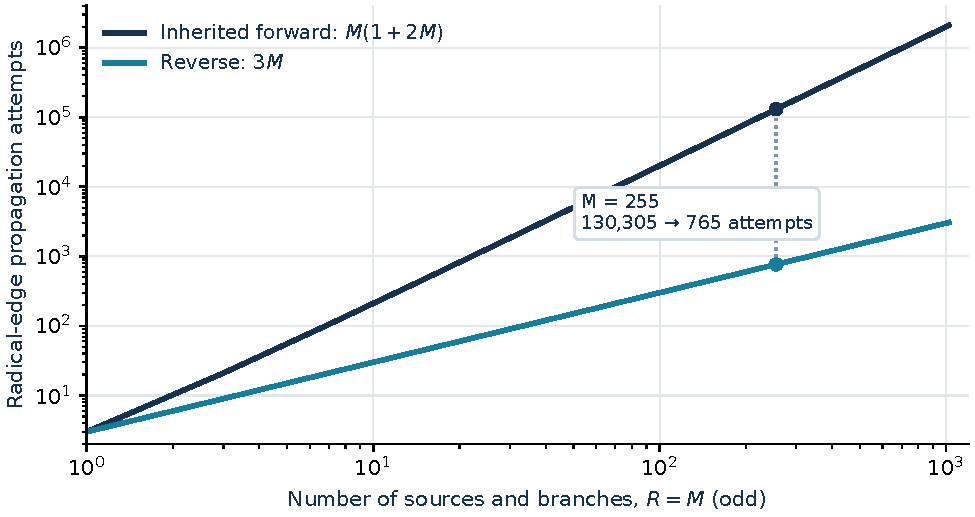
\includegraphics[width=\textwidth]{figures/directional_counts.pdf}
\caption{Exact radical-edge propagation counts for the shared-suffix
family with $R=M$ odd. The curves are the proved formulas, not fitted
timing data. At $M=255$, the ratio is $170\tfrac13$. Scalar setup and
the complete-stage bound are treated separately below.}
\label{fig:directional-counts}
\end{figure}

The counts are edge propagations or radical-edge visits.  They must not be
silently relabelled as cache misses, because many products in this family are
equal.  The implementation's typed identity shortcuts and coefficient caches
can avoid some actual algebra calls.  The repeated coefficient propagation
and accumulation in the forward graph remain, and the theorem states exactly
the operation count that it compares.

These two constructions are valid families of homogeneous algebraic
complexes.  They are not a theorem that arbitrary members arise at an
intermediate stage of scanning a knot diagram.  Establishing such a
realizability result, or finding comparably strong separation families of
actual residual knot diagrams, is a further research question.

\subsection{Compatibility with partial sparse cancellation}

Corridor transfer gives a complete exact alternative after a sparse
cancellation budget is exhausted.  Unlike the earlier support-only shortcut,
it also applies when survivors occupy adjacent degrees and their radical
differential is nonzero.  Because all maps are installed only after the
transfer finishes, the implementation can retain completed sparse pivots and
preserve the current state when a resource exception interrupts the proposed
replacement.  A failed budget or an unsuccessful support certificate is not
a topological verdict.

The operation counts identify two different opportunities: deleting data that
cannot reach a survivor, and avoiding repeated evaluation of a portion shared
by many sources or many targets.  They do not make the scalar survivor
profile smaller.  In particular, they do not resolve the possibility of very
large surviving multiplicities, nor the allocation cost of creating the next
crossing stage.  A general quasi-polynomial complexity theorem still requires
a uniform structural bound beyond the results proved here.

\subsection{Sparse scalar components and the cost of setting up transfer}
\label{sec:sparse-scalar-components}

The transfer counts in Section~\ref{sec:survivor-corridors} do not by themselves
bound the work of constructing $i,p,h$.  The inherited scalar implementation
groups all copies of one shifted matching into binary matrices and returns
columns as integer masks on the complete list of object slots.  A complex
with thousands of disconnected scalar identity pairs can therefore incur
large global masks even though its scalar contraction has only one nonzero
homotopy entry per pair.  That is a representation cost, not an algebraic
necessity.

We remove it by splitting the \emph{scalar} differential graph before doing
binary elimination.  Its vertices are the live original objects, and its
undirected edges are the nonzero entries of $d_0$.  These components are
direct summands of $(C,d_0)$, but usually not of $(C,d)$: radical entries are
deliberately excluded from this graph and may connect different components.
Every scalar component has one matching and one quantum shift, although it
can occupy several homological degrees.

For a singleton $a$, use the contraction with one survivor represented by
$a$, with its inclusion and projection both the identity and its homotopy
zero.  For a component consisting of the single scalar arrow
$a\to b=1$, use no survivor and put $h(b)=a$.  Every larger component is
remapped to its own local object indices, retaining the original relative
order, and processed by the inherited binary contraction.  Its output is
then converted to sorted tuples of nonzero original indices.  Columns of
$i,p,h$ are stored as these sparse tuples, rather than integers whose bit
positions range over all original objects.

\begin{theorem}[Scalar component contraction]
\label{thm:scalar-component-contraction}
The direct sum of the preceding local contractions is a typed special
contraction of $(C,d_0)$.  It preserves matching, quantum shift, and all
identities of Lemma~\ref{lem:corridor-binary}.  Suppose the scalar components
have sizes $\nu_1,\ldots,\nu_r$, and let $\mathcal B$ index those requiring
nontrivial local binary elimination.  The scalar construction admits the
conservative bound
\begin{equation}\label{eq:scalar-component-cost}
 \widetilde O\!\left(N+E+\sum_{j\in\mathcal B}\nu_j^3\right)
\end{equation}
in elementary bit operations, together with
\begin{equation}\label{eq:scalar-component-storage}
 O\!\left(N+\sum_{j\in\mathcal B}\nu_j^2\right)
\end{equation}
stored indices and local matrix entries.  Here $E$ is the number of all
stored differential entries, including radical entries, $N$ counts the original
slots, and the tilde suppresses logarithmic
factors for index manipulation, ordering, and the binary lengths of degree
and type labels.  Singleton and single-arrow components do not contribute a
cubic term.
\end{theorem}

\begin{proof}
The connected components of the scalar graph partition the objects into
subcomplexes, because every nonzero entry of $d_0$ has both endpoints in one
component.  All off-component matrix entries of $d_0$ vanish.  Taking direct
sums of the local identities $pi=1$, $d_0h+hd_0=1+ip$, and the side
conditions proves the corresponding global identities.  Local index changes
do not change matching or quantum shift, and the sparse tuple representation
changes no coefficient.

The scalar graph is constructed by inspecting every stored differential
entry, retaining scalar entries, and joining their endpoints.  The inspection
cost is $O(E)$, even if only a few entries are scalar.  Union by size with
path compression gives the usual
near-linear component calculation; a conservative logarithmic bound also
suffices here.  Each singleton or single arrow is processed in constant
local work and contributes a constant number of nonzero output indices.
For a component of size $\nu_j$, the inherited binary matrix operations have
a conservative cubic bit bound, with quadratic matrix storage.  Mapping
its output supports back to the original indices costs at most a quadratic
number of index operations.  The final ordering and index remapping incur
only the logarithmic factors displayed in~\eqref{eq:scalar-component-cost}.
Summing these costs proves the result.
\end{proof}

Merely taking direct sums would suffice for homotopy correctness, but it
could produce a different homology basis from the frozen reference.  For
entrywise validation of the new transfer we retain that reference basis
exactly.  The following ordering property makes this possible.

\begin{lemma}[Kernel anchors and compatibility of local bases]
\label{lem:scalar-kernel-anchors}
In the frozen scalar algorithm, process source columns in increasing
original object order and reduce them using the highest nonzero target
coordinate.  Every kernel candidate produced by a dependent column has
that column's source index as the largest index in its support.  Call this
index its anchor.  Computing separately on scalar components preserves all
selected kernel representatives, boundary bases, and boundary lifts.
\end{lemma}

\begin{proof}
When source column $a$ is processed, its tracked preimage begins with the
unit vector $e_a$.  Every pivot column available to reduce it was processed
earlier.  Its tracked preimage is supported on those earlier source indices.
Thus reductions can change only coordinates below $a$, and the coordinate
at $a$ stays one.  If the reduced image is zero, the resulting kernel
candidate has largest support index $a$.  Different dependent columns
therefore have different anchors.

For a scalar graph component, every column and tracked preimage is supported
within that component, and its image is supported within the same component
in the next degree.  Pivots from a different component have different target
support and cannot be used in its elimination.  A local remapping that
preserves the original order therefore encounters exactly the same relevant
pivots, in the same order, and constructs exactly the same images, lifts,
and kernel candidates.  Interleaving operations from different components
has no effect on these results.

The later selection of homology representatives starts with the boundary
basis and tests the kernel candidates in source order.  Boundary supports
from other components cannot affect independence in the given component.
The same candidates are consequently selected in both computations.  Finally,
the $B,H,L$ basis inversion is block diagonal with respect to these scalar
components, up to its explicit row and column ordering, so its local inverse
coefficients are also unchanged.
\end{proof}

\begin{corollary}[Exact reproduction of the frozen scalar basis]
\label{cor:scalar-exact-basis}
Merge the local survivor representatives in the order
\begin{equation}\label{eq:scalar-survivor-order}
 (\text{matching},q,h,\text{anchor})
\end{equation}
and remap the survivor indices in $p$ accordingly.  Then the sparse maps
$i,p,h$, converted to ordinary binary columns if desired, are entrywise
identical to the frozen reference maps.
\end{corollary}
\begin{proof}
The reference processes its scalar groups in order $(\text{matching},q,h)$.
Within each group it selects homology representatives in increasing order
of their dependent source columns.  By Lemma~\ref{lem:scalar-kernel-anchors},
that is precisely anchor order and the selected vectors are unchanged by
componentwise computation.  The inclusion columns therefore agree in both
their coefficients and their global order.  The local basis inversions
agree as well; applying the same survivor permutation gives the identical
projection, while the homotopy is independent of survivor numbering.
\end{proof}

The implementation avoids sorting a large list of survivors that already
have the same group key.  It places each representative at its original
anchor index, scans those slots once in increasing order, and appends the
representatives to their $(\text{matching},q,h)$ groups.  It then sorts only
the group keys.  Distinct anchors make the placement unambiguous.  This
also avoids constructing global integer bit masks during the merge.

\subsection{A complete sparse reduction bound for the separation family}
\label{sec:complete-sparse-separation}

The sparse scalar representation can be combined with a less expensive
direction policy.  Instead of constructing a separate packed reachability
label for every endpoint, one first computes two Boolean predicates:
reachable from some input, and able to reach some output.  These suffice to
prune to the corridor.  For a weak component with $a_j$ input ports and $b_j$
output ports, choose forward if $a_j\le b_j$ and reverse otherwise.  The
coarse bound~\eqref{eq:corridor-coarse-propagations} still holds; the fine
endpoint-mask bound is not being computed by this policy.

On general inputs, the port-count policy can make a worse choice than the
fine structural policy because different ports can reach very different
numbers of edges.  Its benefit is that graph setup uses only constant-size
Boolean labels.  Both policies compute the same exact differential and are
available separately so their setup and evaluation costs can be compared.

\begin{theorem}[Complete stage separation at fixed algebra size]
\label{thm:complete-sparse-separation}
Consider the shared-suffix family of
Theorem~\ref{thm:corridor-separation}, with $M$ odd.  Use sparse scalar
components, Boolean corridor pruning, and the port-count direction policy.
The complete reduction of its explicit two-term complex requires
\begin{equation}\label{eq:complete-sparse-family-cost}
 O((R+M)\log(R+M+2))
\end{equation}
word operations and $O(R+M)$ words of working storage, on a word RAM with
words large enough for its object indices.  The old forward evaluation
alone requires $\Omega(RM)$ coefficient-edge propagations.  For $R=M$ odd,
this yields a near-linear versus quadratic separation for the complete
reduction of this algebraic family, without omitting scalar setup.
\end{theorem}

\begin{proof}
The original complex has $N=R+2M+3$ objects, $M+1$ scalar identity edges,
and $R+2M$ radical edges.  Its scalar graph consists of $R+1$ survivor
singletons and $M+1$ single-arrow components.  The direct sparse construction
therefore uses only $R+1$ inclusion entries, $R+1$ projection entries, and
$M+1$ homotopy entries.  There is no nontrivial local binary problem.

The transfer graph has $2R+2M+4$ vertices and $2R+3M+2$ edges.  It is built
in linear work from these sparse supports.  Topological sorting contributes
at most the logarithmic factor in~\eqref{eq:complete-sparse-family-cost};
Boolean reachability and pruning are linear after the order is available;
component finding can be charged at most another linear-logarithmic term,
which is absorbed by the displayed bound. There is a single corridor with $R$ inputs and one
output.  The port policy chooses reverse for $R>1$; when $R=1$ either
direction has the same count.  Reverse evaluation uses $R+2M$ radical-edge
visits and $3M+2R+2$ total propagations, by
Theorem~\ref{thm:corridor-separation}.  It visits each graph vertex once for
the one output root.  All coefficients lie in the fixed eight-dimensional
algebra $\mathbb F_2[x,y,z]/(x^2,y^2,z^2)$, so their operations have constant
word cost.  The input, graph, sparse contraction, working coefficients, and
the $R$ output entries all occupy $O(R+M)$ words.

The inherited forward algorithm performs $R(1+2M)$ radical-edge visits on
this same input.  Even a perfect cache for repeated algebra products does
not remove its repeated propagation and accumulation along those edges.
This gives the stated lower bound and, with $R=M$, the separation.
\end{proof}

This strengthened result concerns the complete reduction of an already
explicit algebraic stage.  It still does not establish the realizability of
this family as knot-scan prefixes, beat the existing minimum-fill Gaussian
algorithm on every such input, or bound the size of every stage produced by
an arbitrary knot diagram.  Those are distinct questions.  Its contribution
is to remove a concrete representation obstruction that would otherwise
invalidate an end-to-end stage claim based only on the transfer counts.
